% to-do
% -----
% - Hogg: should we distinguish parameters (m,b) from their best-fit values?
% - Hogg: should we distinguish = \equiv and \leftarrow ?
% - Hogg: we need to say things about procedure; right now the document is almost entirely about the objective
% - Hogg: should we say something substantial---not superficial---about non-convexity; perhaps initializing trials with RANSAC-like initial conditions
% - Bovy: do something to the fake data that makes PCA differ from the right thing; this requires correlating the variance tensors, I think.

% style notes
% -----------
% - careful with the words ``error'' and ``uncertainty''
% - careful with the words ``probability'' and ``frequency''
% - use () for function arguments, and [] for grouping/precedence
% - define macros; remember 1, 2, infinity

\documentclass[12pt]{article}
\usepackage{amssymb,amsmath,mathrsfs,deluxetable}
\usepackage{natbib}
\usepackage{float,graphicx}
% hypertex insanity
\usepackage{color,hyperref}
\definecolor{linkcolor}{rgb}{0,0,0.25}
\hypersetup{
  colorlinks=true,        % false: boxed links; true: colored links
  linkcolor=linkcolor,    % color of internal links
  citecolor=linkcolor,    % color of links to bibliography
  filecolor=linkcolor,    % color of file links
  urlcolor=linkcolor      % color of external links
}
%%Figure caption
\makeatletter
\newsavebox{\tempbox}
\newcommand{\@makefigcaption}[2]{%
\vspace{10pt}{#1.--- #2\par}}%
\renewcommand{\figure}{\let\@makecaption\@makefigcaption\@float{figure}}
\makeatother

\setlength{\emergencystretch}{2em}%No overflow

\newcommand{\notenglish}[1]{\textit{#1}}
\newcommand{\aposteriori}{\notenglish{a~posteriori}}
\newcommand{\apriori}{\notenglish{a~priori}}
\newcommand{\etal}{et al.}
\newcommand{\eg}{e.g.}

\newcommand{\documentname}{document}
\newcommand{\sectionname}{section}
\newcommand{\equationname}{equation}
\newcommand{\problemname}{Exercise}
\newcommand{\solutionname}{Solution}
\newcommand{\commentsname}{Comments}

\newcounter{problem}
\newenvironment{problem}{\paragraph{\problemname~\theproblem:}\refstepcounter{problem}}{}
\newenvironment{comments}{\paragraph{\commentsname:}}{}

% matrix stuff
\newcommand{\mmatrix}[1]{\boldsymbol{#1}}
\newcommand{\inverse}[1]{{#1}^{-1}}
\newcommand{\transpose}[1]{{#1}^{\scriptscriptstyle \top}}
\newcommand{\mA}{\mmatrix{A}}
\newcommand{\mAT}{\transpose{\mA}}
\newcommand{\mC}{\mmatrix{C}}
\newcommand{\mCinv}{\inverse{\mC}}
\newcommand{\mQ}{\mmatrix{Q}}
\newcommand{\mX}{\mmatrix{X}}
\newcommand{\mY}{\mmatrix{Y}}
\newcommand{\mYT}{\transpose{\mY}}
\newcommand{\mZ}{\mmatrix{Z}}
\newcommand{\vhat}{\mmatrix{\hat{v}}}

% set stuff
\newcommand{\setofall}[3]{\{{#1}\}_{{#2}}^{{#3}}}
\newcommand{\allq}{\setofall{q_i}{i=1}{N}}
\newcommand{\allx}{\setofall{x_i}{i=1}{N}}
\newcommand{\ally}{\setofall{y_i}{i=1}{N}}
\newcommand{\allxy}{\setofall{x_i,y_i}{i=1}{N}}
\newcommand{\allsigmay}{\setofall{\sigma_{yi}^2}{i=1}{N}}
\newcommand{\allC}{\setofall{\mC_i}{i=1}{N}}

% other random multiply used math symbols
\renewcommand{\d}{\mathrm{d}}
\newcommand{\like}{\mathscr{L}}
\newcommand{\pgood}{p_{\mathrm{good}}}
\newcommand{\bperp}{b_{\perp}}
\newcommand{\mean}[1]{\left<{#1}\right>}
\newcommand{\meanZ}{\mean{\mZ}}

\begin{document}
\section*{Data analysis recipes:\ \\
  Fitting a straight line to data\footnote{
    Copyright 2009 David~W.~Hogg (david.hogg@nyu.edu) and Jo Bovy.
    You may copy and distribute this document
    provided that you make no changes to it whatsoever.}}

\noindent
David~W.~Hogg \textsl{and}
Jo~Bovy\\
\textsl{Center~for~Cosmology~and~Particle~Physics, Department~of~Physics,\\
New~York~University}

\begin{abstract}
  We go through all of the considerations involved in fitting a
  straight line to a set of points in a two-dimensional plane.
  Standard chi-squared fitting is only appropriate when there is a
  dimension along which the data points have negligible uncertainties;
  this condition is rarely met in practice.  In addition to
  considering cases of general, heterogeneous, and arbitrarily
  covariant two-dimensional uncertainties, we also look at situations
  in which there are bad data (large outliers), unknown uncertainties,
  and unknown but expected intrinsic scatter in the linear
  relationship being fit.  Above all we emphasize the importance of
  choosing a justified scalar objective, and recommend separating that
  decision from any decisions about the details of optimization.
\end{abstract}

It is conventional to begin any scientific document with an
introduction that explains why the subject matter is important.  Let
us break with tradition and observe that in almost all cases in which
scientists fit a straight line to their data, they are doing something
that is simultaneously \emph{wrong} and \emph{unnecessary}.  It is
wrong because circumstances in which a set of two dimensional
measurements---outputs from an observation, experiment, or
calculation---are truly drawn from a linear relationship is
exceedingly rare.  Indeed, any mildly nonlinear transformation of
coordinates and a truly linear relationship becomes curved.
Furthermore, even if a relationship \emph{looks} linear, unless there
is a confidently held theoretical reason to believe that the data are
generated by a linear relationship, it probably isn't in detail; in
these cases fitting with a linear model can introduce substantial
systematic error.

Even if the investigator doesn't care that the fit is wrong, it is
likely to be unnecessary.  Why?  Because it is rare that, given a
complicated observation, experiment, or calculation, the important
\emph{result} of that work to be communicated forward in the
literature and seminars is the \emph{slope and intercept} of a
best-fit line!  Usually the full distribution of data is much more
rich, informative, and important than any simple metrics made by
fitting an overly simple model.

That said, it must be admitted that one of the most effective ways to
communicate scientific results is with catchy punchlines and compact,
approximate representations, even when those are unjustified and
unnecessary.  For this reason---and in situations where a linear fit
\emph{is} justifiable and essential---the problem of fitting a line to
data comes up very frequently in the life of a scientist.

It is a miracle with which we hope everyone reading this is familiar
that \emph{if} you have a set of two-dimensional points $(x,y)$ that
depart from a perfect, narrow, straight line only by the addition of
gaussian-distributed noise of known amplitudes in one direction (the
$y$ direction without loss of generality), the maximum-likelihood or
best-fit line for the points has a slope $m$ and intercept $b$ that
can be obtained justifiably by a perfectly linear matrix-algebra
operation known as ``least-square fitting''.  This miracle deserves
contemplation.  Once any of the input assumptions is violated (and
note there are many input assumptions), all bets are off, and there
are no consensus methods used by scientists across disciplines.  It is
one of the objectives of this \documentname\ to suggest and promote some
possible consensus methods: We present below simple, straightforward,
comprehensible, and---above all---\emph{justifiable} methods for
fitting a straight line to data with general, non-trivial, and
uncertain properties.

Perhaps because there is no agreed-upon bible or cookbook to turn to,
or perhaps because most investigators would rather make some stuff up
that works ``good enough'' under deadline, or perhaps because many
realize, deep down, that much fitting is really unnecessary anyway,
there are some egregious procedures and associated errors and
absurdities in the literature.  We won't call out the guilty here, but
just make the point to remind everyone that when you cite, rely upon,
or transmit a best-fit slope or intercept reported in the literature,
you may be propagating more noise than signal.

This \documentname\ is part polemic, part attempt at establishing standards,
and part notes for our own future re-use.  We apologize in advance for
some astrophysics bias and failure to review basic ideas of linear
algebra, function optimization, and practical statistics.  Very good
reviews of the latter exist in abundance \citep{jaynes,mackay,press}.
Our focus is on the specific problems of linear fitting that we so
often face; the general ideas appear in the context of these concrete
and relatively realistic example problems.  The reader is encouraged
to do the \problemname s; many of these ask you to produce plots which
can be compared with the \figurename s.

\section{Standard practice}\label{sec:standard}

You have a set of $N>2$ points $(x_i,y_i)$, with known gaussian
uncertainties $\sigma_{yi}$ in the $y$ direction, and no uncertainty
at all (that is, perfect knowledge) in the $x$ direction.  You want to
find the function $f(x)$ of the form
\begin{equation}\label{eq:fofx}
f(x) = m\,x + b \quad ,
\end{equation}
where $m$ is the slope and $b$ is the intercept, that ``best fits''
the points.  What is meant by ``best fits'' is, of course, very
important, and in what follows we will have a lot to say about that.
For now, we describe standard practice:

Construct the matrices
\begin{align}\label{eq:mY}
\mY &= \left[\begin{array}{c}
y_1 \\
y_2 \\
\cdots \\
y_N
\end{array}\right] \quad ,\\
\mA &= \left[\begin{array}{cc}
1 & x_1 \\
1 & x_2 \\
\multicolumn{2}{c}{\cdots} \\
1 & x_N
\end{array}\right] \quad ,\\
\mC & = \left[\begin{array}{cccc}
\sigma_{y1}^{2} & 0 & \cdots & 0 \\
0 & \sigma_{y2}^{2} & \cdots & 0 \\
\multicolumn{4}{c}{\cdots} \\
0 & 0 & \cdots & \sigma_{yN}^{2}
\end{array}\right] \quad ,\label{eq:covar}
\end{align}
where one might call $\mY$ a ``vector'', and the covariance matrix
$\mC$ can be generalized to the case in which there are covariances
between the different $y$-direction uncertainties.  The best-fit
values for the parameters $m$ and $b$ are just the components of a
column vector $\mX$ found by
\begin{equation}\label{eq:lsf}
\left[\begin{array}{c} $b$ \\ $m$ \end{array}\right]
 = \mX = \inverse{\left[\mAT\,\mCinv\,\mA\right]}
  \,\left[\mAT\,\mCinv\,\mY\right] \quad .
\end{equation}
This seems all very complicated, but it is actually the simplest thing
that can be written down that is linear, obeys matrix multiplication
rules, and has the right relative sensitivity to data of different
statistical significance.  It can be justified in one of several ways;
the linear algebra justification starts by noting that you want to
solve the equation
\begin{equation}
\mY = \mA\,\mX \quad ,
\end{equation}
but you can't because that equation is over-constrained.  So you
weight everything with the inverse of the covariance matrix (as you
would if you were doing, say, a weighted average), and then
left-multiply everything by $\mAT$ to reduce the dimensionality, and
then \equationname~(\ref{eq:lsf}) is the solution of that
reduced-dimensionality equation.

This methodology minimizes a quantity $\chi^2$ (``chi-squared''),
which is the total squared error, scaled by the uncertainties, or
\begin{equation}\label{eq:chisquared}
\chi^2
 = \sum_{i=1}^N \frac{\left[y_i - f(x_i)\right]^2}{\sigma_{yi}^2}
 \equiv \transpose{\left[\mY-\mA\,\mX\right]}
 \,\mCinv\,\left[\mY-\mA\,\mX\right]
 \quad ,
\end{equation}
that is, it finds the values for $m$ and $b$ that minimize $\chi^2$.
This, of course, is only one possible meaning of the phrase ``best
fit''; that issue is the main subject of the rest of this
\documentname.

When the uncertainties are gaussian and their variances $\sigma_{yi}$
are correctly estimated, the matrix
$\inverse{\left[\mAT\,\mCinv\,\mA\right]}$ that appears in
\equationname~(\ref{eq:lsf}) is just the covariance matrix (gaussian
uncertainty variances on the diagonal, covariances off the diagonal)
for the parameters in $\mX$.  The justification of this will have to
wait for a discussion of the objective function, if it comes at all.

\begin{comments}
Even when the conditions of standard practice are met, it is
\emph{still} often done wrong!  It is not unusual to see the
individual data-point error estimates ignored, even when they are
known at least approximately.  It is also common for the problem to
get ``transposed'' such that the coordinates for which errors are
negligible are put into the $\mY$ vector and the coordinates for which
errors are \emph{not} negligible are put into the $\mA$ matrix.  In
this latter case, the procedure makes no sense at all really; it
happens when the investigator thinks of some quantity ``really being''
the dependent variable, despite the fact that it has the smaller
error.  For example there are mistakes in the Hubble expansion
literature, because many have an intuition that the ``velocity depends
on the distance'' when in fact velocities are measured better, so from
the point of view of fitting, it is better to think of the distance
depending on the velocity.  In the context of fitting, there is no
meaning to the terms ``independent variable'' and ``dependent
variable'' beyond the error properties of the data.  In performing
this standard fit, the investigator is effectively assuming that the
$x$ values have negligible uncertainties; if they do \emph{not}, then
the investigator is making a mistake.

Conceptually, the inverse covariance matrix appears in the
construction of the $\chi^2$ objective function like a linear
``metric'' for the data space: It is used to turn a $N$-dimensional
vector displacement into a scalar squared distance between the
observed values and the values predicted by the model. This distance
is then minimized.  This idea is sometimes useful for thinking about
statistics as a physicist.

Note that not only does the standard problem solved in this
\sectionname\ have a linear solution, the objective function
``landscape'' is convex so the solution is unique.  This is
remarkable, and almost no perturbation of this problem (as we will see
below) has either of these properties, let alone both.  For this
standard problem, the linearity and convexity permit a one-step
solution with no significant engineering challenges (even when $N$
gets exceedingly large).  As we modify (and make more realistic) this
problem, linearity and convexity will \emph{both} be broken; some
thought will have to be put into the optimization.
\end{comments}

\begin{problem}\label{prob:easy}
Using the standard linear algebra method of this \sectionname, fit the
straight line $y=m\,x+b$ to the $x$, $y$, and $\sigma_y$ values for
data points 5 through 20 in \tablename~\ref{table:data_allerr}.  Make
a plot showing the points, their uncertainties, and the best-fit line.
Your plot should end up looking like \figurename~\ref{fig:easy}.  What
is the standard uncertainty variance $\sigma_m^2$ on the slope of the
line?
\end{problem}

\begin{problem}\label{prob:standard}
Using the standard linear algebra method of this \sectionname, fit the
straight line $y=m\,x+b$ to the $x$, $y$, and $\sigma_y$ values for
all the data points in \tablename~\ref{table:data_allerr}.  Make a
plot showing the points, their uncertainties, and the best-fit line.
Your plot should end up looking like \figurename~\ref{fig:standard}.
What is the standard uncertainty variance $\sigma_m^2$ on the slope of
the line?  Is there anything you don't like about the result?  Is
there anything different about the new points you have included beyond
those used in \problemname~\ref{prob:easy}?
\end{problem}

\begin{problem}\label{prob:quadratic}
Generalize the method of this \sectionname\ to fit a general quadratic
(second order) relationship.  Add another column to matrix $\mA$
containing the values $x_i^2$, and another element to vector $\mX$
(call it $q$).  Then re-do \problemname~\ref{prob:easy} but
fitting for and plotting the best quadratic relationship
\begin{equation}
g(x) = q\,x^2 + m\,x + b \quad.
\end{equation}
Your plot should end up looking like \figurename~\ref{fig:quadratic}.
\end{problem}

\section{The objective function}\label{sec:objective}

A scientist's justification of \equationname~(\ref{eq:lsf}) cannot
appeal purely to abstract ideas of linear algebra, but must originate
from the scientific question at hand.  Here and in what follows, we
will advocate that the only reliable procedure is to use all one's
knowledge about the problem to construct a (preferably) justified,
(necessarily) scalar (or, really, one-dimensional), \emph{objective
  function} that represents monotonically the quality of the fit.  In
this framework, fitting anything to anything involves a scientific
question about the objective function representing ``goodness of fit''
and then a separate and subsequent engineering question about how to
\emph{find the optimum} and, possibly, the confidence interval or
posterior probability distribution around that optimum.  Note that in
the above section we did \emph{not} proceed according to these rules;
indeed the procedure was introduced prior to the objective function,
and the objective function was not justified.

One method for finding or creating a justified scalar objective is to
make a ``generative model'' for the data, or a statistical model for
how a data set similar to the one you have might have been generated.
In the case of the straight line fit in the presence of known,
gaussian uncertainties, one can create this generative model by
imagining that the data \emph{really do} come from a line of the form
$y = f(x) = m\,x+b$, and that the only reason that any data point
deviates from this perfect, straight line is that to this has been
added a small $y$-direction offset drawn from a gaussian distribution
of zero mean and known variance $\sigma_y^2$.  In this model, given an
independent position $x_i$, an uncertainty $\sigma_{yi}$, a slope $m$,
and an intercept $b$, the frequency distribution
$p(y_i|x_i,\sigma_{yi},m,b)$ for $y_i$ is
\begin{equation}\label{eq:objectivei}
p(y_i|x_i,\sigma_{yi},m,b) = \frac{1}{\sqrt{2\,\pi\,\sigma_{yi}^2}}
 \,\exp\left(-\frac{[y_i - m\,x - b]^2}{2\,\sigma_{yi}^2}\right) \quad ,
\end{equation}
where this gives the expected frequency (in a hypothetical set of
repeated experiments) of getting value in the range $[y_i,y_i+\d y]$
per unit $\d y$.

This generative model provides us with a natural, justified, scalar
objective: We seek the line (parameters $m$ and $b$) that maximize the
probability of the observed data or likelihood of the parameters
(which are nearly the same thing in standard parlance).  The
likelihood $\like$ is
\begin{equation}\label{eq:like}
\like \propto \prod_{i=1}^N p(y_i|x_i,\sigma_{yi},m,b) \quad ,
\end{equation}
where we have used ``$\propto$'' not ``$=$'' to be careful about the
infinitesimal volume $(\d y)^N$ and a possible normalization constant
that comes from the overall probability of the data in the context of
the model space (to which we may return below).  Taking the logarithm,
\begin{eqnarray}\displaystyle
\ln\like
 & = & K - \sum_{i=1}^N \frac{[y_i - m\,x - b]^2}{2\,\sigma_{yi}^2} \nonumber\\
 & = & K - \frac{1}{2}\,\chi^2 \quad ,
\end{eqnarray}
where $K$ is some constant.  This shows that likelihood maximization
is identical to $\chi^2$ minimization and we have justified,
scientifically, the procedure of the previous section.

The Bayesian generalization of this is to say that
\begin{equation}
p(m,b|\ally,I) = \frac{p(\ally|m,b,I)}{p(\ally|I)}\,p(m,b|I) \quad ,
\end{equation}
where $m$ and $b$ are the model parameters, $\ally$ is a short-hand
for all the data $y_i$, $I$ is a short-hand for all the prior
knowledge of the $x_i$ and the $\sigma_{yi}$ and everything else about
the problem, $p(m,b|\ally,I)$ is the \emph{posterior} probability
distribution for the parameters given the data and the prior
knowledge, the ratio is the likelihood $\like$ just computed, which
has a frequency distribution for the data on top and that same thing
marginalized over all parameters on the bottom (the denominator can be
thought of as a normalization constant), and $p(m,b|I)$ is the
\emph{prior} probability distribution for the parameters that
represents all knowledge \emph{except} the input data $\ally$.  Unless
the prior $p(m,b|I)$ is pretty informative, the posterior distribution
function $p(m,b|\ally,I)$ here is going to look very similar to the
likelihood function in \equationname~(\ref{eq:like}) above.

We have succeeded in justifying the standard method as optimizing a
justified, scalar objective function.  It is just the great good luck
of Gaussian distributions that that optimization is a pure linear
function of the data, and therefore trivial to implement.

\begin{comments}
In geometry or physics, a ``scalar'' is not just a quantity with a
magnitude; it is a quantity with a magnitude that has certain
transformation properties: It is invariant under some relevant
transformations of the coordinates.  The objective ought to be
something like a scalar in this sense, because we want the inference
to be as insensitive to coordinate choices as possible.  The standard
$\chi^2$ objective function is a scalar in the sense that it is
invariant to translations or rescalings of the data in the $\mY$
vector space defined in \equationname~(\ref{eq:mY}).  Of course a
\emph{rotation} of the data in the space would be pretty strange, and
would make the covariance matrix $\mC$ much more complicated, so
perhaps the fact that the objective is literally a linear algebra
scalar---this is clear from its matrix representation in
\equationname~(\ref{eq:chisquared})---is a red herring.

The more important thing about the objective is that it must have
\emph{one magnitude only}.  Often when one asks a scientist what they
are trying to optimize, they will tell you something like ``I am
trying to maximize the resolution, minimize the noise, and minimize
the error in measured fluxes''.  Well, those are good objectives, but
\emph{you can't optimize them all}.  You either have to pick one, or
make a convex combination of them (such as by adding them together in
quadrature with weights).  This point is so obvious, it is not clear
what else to say, except that many scientific investigations are so
ill-posed that the investigator does not know what is being optimized.

We have tried in this \documentname\ to be a bit careful with words.
Following \citet{jaynes}, we have tried to use the word
``probability'' for our knowledge or uncertainty about a parameter in
the problem, and ``frequency'' for the rate at which a random variable
comes a particular way.  So the noise process that sets the
uncertainty $\sigma_{yi}$ has a frequency distribution, but if we are
just talking about our \emph{knowledge} about the true value of $y$
for a data point measured to have value $y_i$, we might describe that
with a probability distribution.  In the Bayesian context, then---to
get extremely technical---the posterior probability distribution
function is truly a probabiity distribution, but the likelihood factor
is constructed from frequency distributions.  This relates to the
difference between ``uncertainty'' and ``error''; if your data have
\emph{errors}, correct them!  Your data come with
\emph{uncertainties}, which are limitations to your knowledge, not
\emph{mistakes}.

One oddity in this \sectionname\ is that when we set up the Bayesian
problem we put the $\allx$ and $\allsigmay$ into the prior information
$I$ and \emph{not} into the data.  These were not considered data.
Why not?  This was a choice, but we made it to emphasize that in the
standard approach to fitting, there is a \emph{total asymmetry}
between the $x_i$ and the $y_i$.  The $x_i$ are considered part of the
\emph{experimental design}; they are the input to an experiment that
got the $y_i$ as output.  For example, the $x_i$ are the times
(measured by your perfect and reliable clock) at which you chose
\apriori\ to look through the telescope, and the $y_i$ are the Right
Ascensions you measured at those times.  As soon as there is any sense
in which the $x_i$ are themselves \emph{also} data, the
method---Bayesian or frequentist---of this \sectionname\ is invalid.

It remains a miracle (to us) that the optimization of the $\chi^2$
objective, which is the only sensible objective under the assumptions
of the standard problem, has a linear solution.  One can attribute
this to the magical properties of the gaussian distribution, but the
gaussian distribution is also the maximum entropy distribution (the
least informative possible distribution) constrained to have zero mean
and a known variance; it is the limiting distribution of the central
limit theorem.  That this leads to a convex, linear algebra solution
is something for which we all ought to give thanks.
\end{comments}

\begin{problem}
Imagine a set of $N$ measurements $t_i$, with uncertainty variances
$\sigma_{ti}^2$, all of the same (unknown) quantity $T$.  Assuming the
generative model that each $t_i$ differs from $T$ by a
gaussian-distributed offset, taken from a gaussian with zero mean and
variance $\sigma_{ti}^2$, write down an experession for the log
likelihood $\ln\like$ for the data given the model parameter $T$.
Take a derivative and show that the maximum likelihood value for $T$
is the usual weighted mean.
\end{problem}

\begin{problem}
Take the matrix formulation for $\chi^2$ given in
\equationname~(\ref{eq:chisquared}) and take derivatives to show that
the minimum is at the matrix location given in
\equationname~(\ref{eq:lsf}).
\end{problem}

\section{Robustness to outliers}\label{sec:robust}

The standard linear fitting method is very sensitive to
\emph{outliers}, points that are substantially farther from the linear
relation than expected because of unmodeled experimental error or
unmodeled but rare sources of noise.  There are two general approaches
to this problem, which are not necessarily different.  The first is to
``soften'' the objective function at large deviation.  The second is
to find ways to objectively remove or reject ``bad'' points.  Both of
these are strongly preferable to sorting through the data by hand, for
reasons of subjectivity and irreproducibility that we need not state.

One straightforward way to soften the objective function relative to
$\chi^2$ is to lower the power to which residuals are raised.  For
example, if we model the frequency distribution
$p(y_i|x_i,\sigma_{yi},m,b)$ not with a gaussian but rather with a
biexponential
\begin{equation}
p(y_i|x_i,\sigma_{yi},m,b) = \frac{1}{2\,s_i}
 \,\exp\left(-\frac{|y_i-m\,x_i-b|}{s_i}\right) \quad ,
\end{equation}
where $s_i$ is an estimate of the mean absolute error, probably
correctly set to something like $s_i\approx \sigma_{yi}$.
Optimization of the total log likelihood is equivalent to minimizing
\begin{equation}\label{eq:biexp}
X = \sum_{i=1}^N \frac{|y_i-f(x_i)|}{s_i} \quad ,
\end{equation}
where $f(x)$ is the straight line of \equationname~\ref{eq:fofx}.
This approach is rarely quantitatively justified, but it has the nice
property that it introduces no new parameters.

Another straightforward softening is to (smoothly) cut off the
contribution of a residual as it becomes large.  For example, replace
$\chi^2$ with
\begin{equation}\label{eq:soft}
\chi_Q^2 = \sum_{i=1}^N \frac{Q^2\,[y_i-f(x_i)]^2}
  {Q^2\,\sigma_{yi}^2+[y_i-f(x_i)]^2} \quad ,
\end{equation}
where $Q^2$ is the maximum amount a point can contribute to $\chi_Q^2$
 \citep{hampel}.  When each residual is small, its
contribution to $\chi_Q^2$ is nearly identical to its contribution to
the standard $\chi^2$, but as the residual gets substantial, the
contribution of the residual does not increase as the square.  This is
about the simplest robust method that introduces only one new
parameter ($Q$).

In both of these softenings of $\chi^2$, the objective function is no
longer purely quadratic, and the solution is no longer purely linear.
Worse, in almost any reasonable softening, the problem becomes
\emph{non-convex}; that is, there will, in general, be multiple optima
from which the global optimum must be selected.  These two problems
are both in the area of \emph{optimization}, a sensible discussion of
which is \emph{way} beyond the scope of this \documentname\
\citep[see, \eg,][]{press}.  However, we can provide a bit of advice.

The first piece of advice is to find, get used to, and take care of
some good non-linear optimizer or optimization code.  It will be
necessary in all your inference.  Most data analysis platforms have
optimizers that can handle problems like those presented here with
little or no trouble.  The second piece of advice is to spend a bit of
thought on initialization.  That is, do not start the optimizer in an
arbitrary point in parameter space, but rather initialize it near
where you think the answer is likely to be, using either your prior
knowledge, or else a linear fit (which provides an objective starting
point).  The third piece of advice is to check for multiple minima by
randomly sampling parameter space in some significant region around
the optimum you have, re-converge the nonlinear optimizer, and verify
that you return to the same best optimum, or that if you come to a
different one, it has a worse value for the objective.

One attractive kind of optimizer is a sampler such as a Markov Chain
Monte Carlo method \citep{mackay}.  These take a bit of getting used
to, but once you have them working well, they handle the optimization
and the local minima problems simultaneously.  These only have
well-defined properties when your objective function can be
interpreted as a probability or likelihood, but that is okay here.  In
the Bayesian scheme below, they simultaneously find your best fit
parameters \emph{and} provide a sampling from the posterior
distribution function, a Good Thing to carry forward (as we note
below).

The alternative to these softenings is to try data rejection, in which
we add to the problem a set of $N$ binary integers $q_i$, one per data
point, each of which is unity if the $i$th data point is good, and
zero if the $i$th data point is bad (cite Press and Jaynes here).  In
addition, to construct an objective function one needs an additional
parameter $\pgood$, which is the \emph{prior} probability that any
individual data point is good.  All these $N+1$ extra parameters may
seem like crazy baggage, but their values can be \emph{inferred} and
\emph{marginalized out} so in the end, this method introduces \emph{no
 new parameters}.

In this situation, we don't know a consistent way to proceed that isn't
Bayesian (possibly for lack of trying), so let's go Bayesian.  In this
case, likelihood is
\begin{eqnarray}\displaystyle
\frac{p(\ally|m,b,\allq,\pgood,I)}{p(\ally|I)}
 &\propto& \prod_{i=1}^N \left[\exp\left(-\frac{[y_i-m\,x_i-b]^2}{2\,\sigma_{yi}^2}\right)\right]^{q_i} \quad ,
\end{eqnarray}
but there is an important prior probability
\begin{eqnarray}\displaystyle
p(m,b,\allq,\pgood|I)
 &=& p(m,b|I)\,p(\allq|\pgood,I)\,p(\pgood|I) \nonumber \\
 &=& p(m,b|I)\,\pgood^{q_i}\,[1-\pgood]^{[1-q_i]} \quad ,
\end{eqnarray}
where we have assumed that the prior probability distribution
$p(\pgood|I)$ for $\pgood$ is just flat on the interval $0<\pgood<1$
(the least informative possible assumption).

The posterior probability distribution is the product of the
(correctly normalized) likelihood times the prior.  If all we care
about are the parameters $(m,b)$ of the line, we have to marginalize
the posterior probability distribution over all choices for the binary
integers $\allq$ and all possible values for $\pgood$.  This
marginalization involves evaluating and marginalizing (over $\pgood$)
$2^N$ different likelihoods!  Of course because very few points are
true candidates for rejection, there are many ways to ``trim the
tree'' and do this quickly; the lazy can simply sample; the very lazy
can loop over all $2^N$ and go on vacation while it executes.

One unfortunate (though unavoidably correct) thing about any Bayesian
method is that it does not return an ``answer'' but rather it returns
a \emph{posterior probability distribution}.  Strictly, this posterior
distribution function \emph{is} your answer.  However, what scientists
are usually doing is not, strictly, inference, but rather,
decision-making.  That is, the investigator wants an answer, not a
distribution.  There are (at least) two reactions to this.  One is to
ignore the fundamental Bayesianism at the end, and choose simply the
``maximum \aposteriori'' (MAP) answer---the single value of $(m,b)$
that optimizes the fully marginalized (over $\pgood$ and $\allq$)
posterior probability distribution function.  This is the Bayesian's
analog of maximum likelihood.  The other reaction is to suck it up and
sample the posterior probability distribution and carry forward not
one answer to the problem but $M$ answers, each of which is drawn
fairly and independently from the posterior distribution function.
The latter is to be preferred because \textsl{(a)}~it shows the
uncertainties very clearly, and \textsl{(b)}~the sampling can be
carried forward to future inferences as an approximation to the
posterior distribution function, useful for propagating uncertainty,
or standing in as a \emph{prior} for some subsequent inference.

Another unfortunate (though unavoidably correct) thing about any
Bayes\-ian method is that prior probabilities must be specified.  In any
situation of straight-line fitting where the data are good, these
priors do not matter very much to the final answer.  The way we have
written our likelihoods, the MAP result becomes very directly
analogous to the maximum likelihood answer when the (improper,
non-normalizable) prior ``flat in $m$, flat in $b$'' is adopted.
Usually the investigator \emph{does} have some basis for setting some
more informative priors, but a deep and sensible discussion of priors
is beyond the scope of this \documentname.

\begin{comments}
Because, in this \sectionname, we have broken the assumptions of
least-square fitting, we have also broken the linearity and convexity
of the problem.  That is, no robust procedure will be linear, and not
many robust procedures can be convex, so everything in the category of
modifying $\chi^2$ must be iterated to convergence.  In the Bayesian
scheme presented above, there is no iteration to convergence, but
there is a marginalization over a large discrete space.  Even these
minimal modifications to the standard assumptions ruin the miracle of
linear least squares; this shows how unusual and special the
``textbook'' case is.

Importantly, the \emph{scientific} decision is about the objective
function.  Optimization is an \emph{engineering} consideration.  This
distinction is not made to denigrate the latter (we are very much
engineers); it is to emphasize that optimizers should be chosen on
practical grounds of time, resources, and availability.

When flagging bad data, you might not want to give all points the same
prior probability distribution function over $\pgood$, though it is
rare that one has reliable information about the unreliability of
one's data.  Complementary to this, one of the amusing things about
the Bayesian posterior developed above is that you can pick a
particular data point $J$ and marginalize over $(m,b)$ and all the
$q_i$ \emph{except} $q_J$.  This will return the marginalized
posterior probability that point $J$ is good.  This is good for
embarassing colleagues in meta-analyses (cite Press here).

The standard method for removing sensitivity to outliers (in
astrophysics, anyway) is known as ``sigma-clipping''.  This is a
procedure that involves performing the fit, identifying the worst
outliers in a $\chi^2$ sense---the points that contribute more than
some threshold $Q^2$ to the $\chi^2$ sum, removing those, fitting
again, identifying again, and so on to convergence.  This procedure is
easy to implement, fast, and reliable (provided that the threshold
$Q^2$ is set high enough), but it has various problems that make it
less suitable than the methods described above.  One is that it is a
\emph{procedure} not an \emph{objective function}.  The procedure does
not necessarily optimize a justifiable objective.  A second is that
the procedure gives an answer that depends, in general, on the
starting point or initialization, and because there is there is no way
to compare different answers (there is no objective function), the
investigator can't decide which of two converged answers is
``better''.  You might think that the answer with least scatter
(smallest $\chi^2$ per data point) is better, but that will favor
solutions that involve rejecting most of the data; you might think the
answer that uses the most data is better, but that can have a very
large $\chi^2$.  These issues relate to the fact that the method does
not explicitly \emph{penalize} the rejection of data; this is another
bad consequence of not having an explicit objective function.  A third
problem is that the procedure does not necessarily converge to
anything non-trivial at all; if the threshold $Q^2$ gets very small,
there are situations in which all but two of the data points can be
rejected by the procedure.  All that said, with a large $Q^2$ and
standard, pretty good data, the sigma-clipping procedure is easy to
implement and fast; we have often used it ourselves.

One extremely common variation on the problem of data rejection is the
situation in which you have to perform data rejection but you
\emph{don't know the magnitudes of your uncertainties} $\allsigmay$.
We will say a bit more about this in \sectionname~\ref{sec:goodness},
but the general procedure is to include the $\allsigmay$ as model
parameters and infer them and marginalize over them \emph{also}.  This
is much more tractable and pleasant if you can assume that all the
data-point uncertainties are comparable or you know something else
equally informative about their \emph{relative} magnitudes.

Hogg: Consider either here or above some kind of foreground/background
EM modeling, a la Dustin.
\end{comments}

\begin{problem}\label{prob:biexp}
Using the biexponential objective function of
\equationname~(\ref{eq:biexp}), find the best-fit straight line
$y=m\,x+b$ for the $x$, $y$, and $\sigma_y$ values in
\tablename~\ref{table:data_allerr}.  You will have to use a non-linear
optimizer of some kind or you will have to take a sampling approach.
Make a plot showing the points, their uncertainties, and the best-fit
line.  The results using a few of the optimization methods are shown
in \figurename s~\ref{fig:biexpa} through \ref{fig:biexpc}. How does
this compare to the standard result you obtained in
\problemname~\ref{prob:standard}?  Do you like it better or worse?
\end{problem}

\begin{problem}\label{prob:softchisq}
Using the soft chi-squared objective function of
\equationname~(\ref{eq:soft}), find the best-fit straight line
$y=m\,x+b$ for the $x$, $y$, and $\sigma_y$ values in
\tablename~\ref{table:data_allerr}.  You will have to use a non-linear
optimizer of some kind or you will have to take a sampling approach.
Alternatively, you can try an iterated-linear method in which you
iterate the standard linear method but modify the weights at each
iteration.  Make a plot showing the points, their uncertainties, and
the best-fit line.  The results using a few of the optimization
methods are shown in \figurename s~\ref{fig:softchisqa} through
\ref{fig:softchisqd}. How does this compare to the standard result you
obtained in \problemname~\ref{prob:standard}?  Do you like it better
or worse?
\end{problem}

\begin{problem}
Using the fully marginalized Bayesian data rejection method described
above, find the best-fit (the maximum \aposteriori) straight line
$y=m\,x+b$ for the $x$, $y$, and $\sigma_y$ values in
\tablename~\ref{table:data_allerr}.  Before choosing the MAP line,
marginalize over $\pgood$ and $\allq$ by (dumbly) looping over every
possible (non-trivial) assigment of $q_i$ values, and at each
assignment, integrate over all possible values of $\pgood$.  Make a
plot showing the points, their uncertainties, and the MAP line.  How
does this compare to the standard result you obtained in
\problemname~\ref{prob:standard}?  Do you like the MAP line better or
worse?  For extra credit, plot a sampling of 10 lines drawn from the
marginalized posterior distribution for $(m,b)$ (marginalized over
$\pgood$ and $\allq$) and plot the samples as a set of light grey or
transparent lines.  For extra extra credit, mark each data point on
your plot with the fully marginalized probability that the point is
good (that is, not rejected, or has $q=1$).
\end{problem}

\section{Goodness of fit and unknown data uncertainties}\label{sec:goodness}

How can you decide if your fit is a good one, or that your assumptions
are justified?  And how can you infer or assess the individual
data-point uncertainties if you don't know them, or don't trust them?
These problems are related problems, but they are coupled: In the
standard (frequentist) paradigm, you can't test your assumptions
unless you are very confident about your uncertainty estimates, and
you can't test your uncertainty estimates unless you are very
confident about your assumptions.

Imagine that the generative model in \sectionname~\ref{sec:objective}
is a valid description of the data.  In this case, the noise
contribution for each data point $i$ has been drawn from a gaussian
with variance $\sigma_{yi}^2$.  In this case, the expectation is that
data point $i$ will provide a mean squared error comparable to
$\sigma_{yi}^2$, and a contribution of roughly unity to $\chi^2$ when
the parameters $(m,b)$ are set close to their true values.  Because in
detail there are two fit parameters $(m,b)$ which you have been
permitted to optimize, the expectaton for $\chi^2$ is smaller than
$N$. Because the model is linear, the distribution of $\chi^2$ is
known analytically and is given (unsurprisingly) by a
\emph{chi-square} distribution: in the limit of large $N$ the rule of
thumb is that---when the model is a good fit and the uncertainties are
gaussian with known variances,
\begin{equation}
\chi^2 = [N-2] \pm \sqrt{2[N-2]} \quad ,
\end{equation}
where the $\pm$ symbol is used loosely to indicate something close to
a standard error (something close to a 68-percent confidence
interval).  If you find $\chi^2$ in this ballpark, it is conceivable
that the model is good.

Model rejection on the basis of too-large $\chi^2$ is a frequentist's
option only.  A Bayesian can't interpret the data without a model, so
there is no meaning to the question ``is this model good?''.
Bayesians only answer questions of the form ``is this model better
than that one?''.  Because we are only considering the straight-line
model in this \documentname, further discussion of this point goes beyond
our scope (aside from a few comments below).

It is easy to get a $\chi^2$ much \emph{higher} than $[N-2]$; getting
a \emph{lower} value seems impossible; yet it happens very frequently.
This is one of the many reasons that rejection or acceptance of a
model on the $\chi^2$ basis is dangerous; exactly the same kinds of
problems that can make $\chi^2$ unreasonably low can make it
unreasonably high; worse yet, it can make $\chi^2$ reasonable when the
model is bad.  Reasons $\chi^2$ can be lower include that uncertainty
estimates are often underestimated, and, worse, often positively
correlated.  The opposite of these problems can make $\chi^2$ high
when the model is good.

Correlated measurements are not uncommon; the process by which the
observations were taken often involve shared information or
assumptions. If the individual data-point uncertainties have been
estimated by some means that effectively marginalizes over some or all
of that shared information, then there will be large covariances among
the data points.  These covariances bring off-diagonal elements into
the covariance matrix $\mC$, which was trivially constructed in
\equationname~(\ref{eq:covar}) under the assumption that all
covariances (off-diagonal elements) are precisely zero.  Once the
off-diagonal elements are non-zero, $\chi^2$ must be computed by the
matrix expression in \equationname~(\ref{eq:chisquared}); this is
equivalent to replacing the sum over $i$ to two sums over $i$ and $j$
and considering all cross terms
\begin{equation}
\chi^2 =
 \transpose{\left[\mY-\mA\,\mX\right]}\,\mCinv\,\left[\mY-\mA\,\mX\right]
 = \sum_{i=1}^N \sum_{j=1}^N
 \frac{\left[y_i-f(x_i)\right]\,(\mCinv)_{ij}[y_j-f(x_j)]}
 {\sigma_{yij}} \quad,
\end{equation} 
where the $(\mCinv)_{ij}$ are the elements of the inverse covariance matrix.

In principle, data-point uncertainty variance underestimation or mean
point-to-point covariance can be \emph{estimated} by adjusting them
until $\chi^2$ is reasonable, in a model you know (for independent
reasons) to be good.  This is rarely a good idea, both because you
rarely know that the model is a good one, and you are much better
served \emph{understanding} your variances and covariances directly.

If you don't have or trust your uncertainty estimates and don't care
about them at all, your best bet is to go Bayesian, infer them, and
marginalize them out.  Imagine that you don't know anything about your
individual data-point uncertainty variances $\allsigmay$ at all.
Imagine, further, that you don't even know anything about their
\emph{relative} magnitudes; that is, you can't even assume that they
have similar magnitudes.  In this case a procedure is the following:
Move the uncertainties into the model parameters to get the large
parameter list $(m,b,\allsigmay)$.  Pick a prior on the uncertainties
(on which you must have \emph{some} prior information, given, for
example, the range of your data and the like).  Apply Bayes's rule to
obtain a posterior distribution function for all the parameters
$(m,b,\allsigmay)$.  Marginalize over the uncertainties to obtain the
properly marginalized posterior distribution function for $(m,b)$.  No
sane person would imagine that the procedure described here can lead
to any informative inference.  However, if the prior on the
$\allsigmay$ is relatively flat in the relevant region, the \emph{lack
  of specificity} of the model when the uncertainties are large pushes
the system to smaller uncertainties, and the \emph{inaccuracy} of the
model when the uncertainties are small pushes the system to larger
uncertainties.  If the model is reasonable, the inferred uncertainties
will be reasonable too.

\begin{comments}
Frequentist model rejection on the basis of unnacceptable $\chi^2$
should not be confused with model \emph{comparison} performed with
$\chi^2$.  If $\chi^2$ differs from the the number of degrees of
freedom ($N-2$ here) by something on the order of the square root of
that, the model cannot be rejected on a $\chi^2$ basis.  However, if
two equally plausible models differ from one another by a difference
$\Delta\chi^2$ substantially larger than unity, the model with the
lower $\chi^2$ can be preferred and the higher rejected on that basis,
even if the higher still shows an acceptable $\chi^2$.  This
difference between model rejection and model comparison is
counterintuitive, but it emerges from the difference that in the moel
comparison case, there are \emph{two} models, not one, and they are
both (by assumption) equally plausible \apriori.  The fact that both
models are reasonable does not mean that we cannot prefer the more
reasonable one. The conditions for model comparison are stronger, so
the test is more sensitive.

In the case of correctly estimated uncertainty variances and two
models that are equally plausible \apriori, the $\Delta\chi^2$ value
between the models is (twice) the natural logarithm of the odds ratio
between the models.  For this reason, large $\Delta\chi^2$ values
generate considerable confidence.

Hogg: Something about Bayesian model selection and decision theory?
\end{comments}

\begin{problem}
Assess the $\chi^2$ value for the fit performed in
\problemname~\ref{prob:easy} (do that problem first if you haven't
already).  Is the fit good?
\end{problem}

\begin{problem}
Re-do the fit of \problemname~\ref{prob:easy} but setting all
$\sigma_{yi}^2=S$, that is, ignoring the uncertainties and replacing
them all with the same value $S$.  Now what uncertainty variance $S$
would make $\chi^2 = N-2$?  How does it compare to the mean and median
of the uncertainty variances $\allsigmay$?
\end{problem}

\begin{problem}
Flesh out and write all equations for the Bayesian uncertainty
estimation and marginalization procedure described in this
\sectionname.  Note that the inference and marginalization would be
very expensive without excellent sampling tools!  Make the additional
(unjustified) assumption that all the uncertainties have the same
variance $\sigma_{yi}^2=S$ to make the problem tractable.  Apply the
method to the $x$ and $y$ values for points 5 through 20 in
\tablename~\ref{table:data_allerr}.  Make a plot showing the points,
the maximum \aposteriori\ value of the uncertainty variance as error
bars, and the maximum \aposteriori\ straight line.  For extra credit,
plot two straight lines, one that is maximum \aposteriori\ for the
full posterior and one that is the same but for the posterior after
the uncertainty variance $S$ has been marginalized out.  Also plot two
sets of error bars, one that shows the maximum for the full posterior
and one for the posterior after the line parameters $(m,b)$ have been
marginalized out.
\end{problem}

\section{Assigning uncertainties to best-fit parameters}\label{sec:uncertainty}

In the standard linear-algebra method of $\chi^2$ minimization given
in \sectionname~\ref{sec:standard}, the uncertainties in the best-fit
parameters $(m,b)$ are given by the two-dimensional output covariance
matrix
\begin{equation}
\left[\begin{array}{cc}
\sigma_{b}^2 & \sigma_{mb} \\
\sigma_{mb} & \sigma_{m}^2
\end{array}\right] = \inverse{\left[\mAT\,\mCinv\,\mA\right]} \quad ,
\end{equation}
where the ordering is defined by the ordering in matrix $\mA$. The
justification for this is given by simple propagation of uncertainties
and only for large $N$ are these uncertainties gaussian. But these
best-fit uncertainties \emph{only} strictly hold under three extremely
strict conditions, almost none of which is met in real practice:
\textsl{(a)}~The uncertainties in the data points must truly be
gaussian, with variances correctly described by the $\sigma_{yi}^2$,
\textsl{(b)}~there must be no rejection of any data or any departure
from the exact, standard definition of $\chi^2$ given in
\equationname~(\ref{eq:chisquared}), and \textsl{(c)}~the generative
model of the data implied by the method---that is, that the data are
truly drawn from a negligible-scatter linear relationship and
subsequently had noise added, where the noise offsets were generated
by a gaussian process---must be an accurate description of the data.

These conditions are rarely met in practice.  Often the noise
estimates are rough (or missing entirely!), the uncertainties are
known not to be gaussian, the investigator has applied data rejection
or equivalent conditioning, and the relationship has intrinsic scatter
and curvature.  For these generic reasons, we much prefer empirical
estimates of the uncertainty in the best-fit parameters.

In the Bayesian scheme of \sectionname~\ref{sec:robust}, the output is
a posterior distribution for the parameters $(m,b)$.  This
distribution function is, in the sense we are using it here, an
empirical measurement of the uncertainties of the parameters.  The
uncertainty variances $(\sigma_m^2,\sigma_b^2)$ and the covariance
$\sigma_{mb}$ can be computed as second moments of this posterior
distribution function.  Computing the variances this way does involve
assumptions, but it does \emph{not} involve any assumption that the
model is a good fit to the data; that is, as the model becomes a bad
fit to the data (for example when the data points are not consistent
with being drawn from a narrow, straight line), these uncertainties
change in accordance.  That is in strong contrast to the elements of
the matrix $\inverse{\left[\mAT\,\mCinv\,\mA\right]}$, which don't
depend in any way on the quality of fit.

In any non-Bayesian scheme, or when the full posterior has been
discarded in favor of only the MAP value, there are still empirical
methods for determining the uncertainties in the best-fit parameters.
The two most common are \emph{bootstrap} and \emph{jackknife}.  The
first attempts to empirically create new data sets that are similar to
your actual data set.  The second measures your differential
sensitivity to each individual data point.

In bootstrap, you do the unlikely-sounding thing of drawing $N$ data
points randomly from the $N$ data points you have \emph{with
  replacement}.  That is, some data points get dropped, and some get
doubled, but the important thing is that you select each of the $N$
that you are going to use in each trial independently from the whole
set of $N$ you have.  You do this selection of $N$ points once for
each of $M$ bootstrap trials $j$.  For each of the $M$ trials $j$, you
get an estimate---by whatever method you are using (linear fitting,
fitting with rejection, optimizing some custom objection
function)---of the parameters $(m_j,b_j)$, where $j$ goes from $1$ to
$M$.  An estimate of your uncertainty variance on $m$ is
\begin{equation}
\sigma_m^2 = \frac{1}{M}\,\sum_{j=1}^M [m_j-m]^2 \quad ,
\end{equation}
where $m$ stands in for the best-fit $m$ using all the data.  The
uncertainty variance on $b$ is the same but with $[b_j-b]^2$ in the
sum, and the covariance $\sigma_{mb}$ is the same but with
$[m_j-m]\,[b_j-b]$.  Bootstrap creates a new parameter, the number $M$
of trials.  There is a huge literature on this, so we won't say
anything too specific, but one intuition is that once you have $M$
comparable to $N$, there probably isn't much else you can learn,
unless you got terribly unlucky with your random number generator.

In jackknife, you make your measurement $N$ times, each time
\emph{leaving out} data point $i$.  Again, it doesn't matter what
method you are using, for each leave-one-out trial $i$ you get an
estimate $(m_i,b_i)$ found by fitting with all the data \emph{except}
point $i$.  Then your best-fit slope becomes
\begin{equation}
m = \frac{1}{N}\,\sum_{i=1}^N m_i \quad ,
\end{equation}
and the uncertainty variance becomes
\begin{equation}
\sigma_m^2 = \frac{N-1}{N}\,\sum_{i=1}^N [m_i-m]^2 \quad ,
\end{equation}
with the obvious modifications to make $\sigma_b^2$ and
$\sigma_{mb}$.  The factor $[N-1]/N$ accounts, magically, for the
fact that the samples are not independent in any sense, and can only
be justified in the limit that everything is gaussian and all the
points are identical in their error properties.

\begin{comments}
Hogg: Compare jackknife and bootstrap in terms of ``conservativeness''.
Note that neither makes sense if there is a large dynamic range in the
$\sigma_{yi}^2$.  Why do these techniques have the names they do?
They are extremely useful when you don't know or don't trust your
uncertainties $\allsigmay$.

If you are doing sigma-clipping or anything that looks like standard
least-square fitting but with small modifications, it might be
tempting to use the standard uncertainty estimate.  But that is
definitely wrong, because whatever encouraged you to do the
sigma-clipping or other modifications is probably sufficient reason to
disbelieve the standard uncertainty estimate.

Hogg: Don't we have examples where a bad-fitting model can lead to very
tight Bayesian constraints; that is, aren't we being too nice to the
Bayesians?
\end{comments}

\begin{problem}
Compute the standard uncertainty $\sigma_m^2$ obtained for the slope
of the line found by the standard fit you did in
\problemname~\ref{prob:standard}.  Now make jackknife (20 trials) and
bootstrap estimates for the uncertainty $\sigma_m^2$.  How do the
uncertainties compare and which seems most reasonable, given the data
and uncertainties on the data?
\end{problem}

\section{Arbitrary two-dimensional uncertainties}\label{sec:twod}

Of course most real two dimensional data $\allxy$ come with
uncertainties in \emph{both} directions (both $x$ and $y$).  You might
not \emph{know} the amplitudes of these uncertainties, but it is
unlikely that the $x$ values are known to sufficiently high accuracy
that \emph{any} of the straight-line fitting methods given so far is
valid.  Recall that everything so far has assumed that the
$x$-direction uncertainties were negligible.

In general, when one makes a two dimensional measurement $(x_i,y_i)$,
that measurement comes uncertainties $(\sigma_{xi}^2,\sigma_{yi}^2)$
in both directions, and some covariance $\sigma_{xyi}$ between them.
These can be put together into a covariance tensor $\mC_i$
\begin{equation}
\mC_i = \left[\begin{array}{cc}
\sigma_{xi}^2 & \sigma_{xyi} \\ \sigma_{xyi} & \sigma_{yi}^2
\end{array}\right] \quad .
\end{equation}
If the errors are gaussian, or if all that is known about the
uncertainties is their variances, then the covariance tensor can be
used in a two-dimensional gaussian representation of the probability
of getting measurement $(x_i,y_i)$ when the ``true value'' (the value
you would have for this data point if it had been observed with
negligible error) is $(x,y)$:
\begin{equation}
p(x_i,y_i|\mC_i,x,y) = \frac{1}{2\,\pi\,\det(\mC_i)^{\frac{1}{2}}}
  \,\exp\left(-\frac{1}{2}\,\transpose{\left[\mZ_i - \mZ\right]}
  \,\inverse{\mC_i}\,\left[\mZ_i - \mZ\right]\right) \quad ,
\end{equation}
where we have implicitly made column vectors
\begin{equation}\label{eq:mZ}
\mZ = \left[\begin{array}{c} x \\ y \end{array}\right] \quad ; \quad
\mZ_i = \left[\begin{array}{c} x_i \\ y_i \end{array}\right] \quad .
\end{equation}

Now in the face of these general (though gaussian) two-dimensional
uncertainties, how do we fit a line?  Justified objective functions
will have something to do with the probability of the observations
$\allxy$ given the uncertainties $\allC$, as a function of properties
$(m,b)$ of the line.  As in \sectionname~\ref{sec:objective}, the
probability of the observations given model parameters $(m,b)$ is
proportional to the \emph{likelihood} of the parameters given the
observations.  We will now construct this likelihood and maximize it,
or else multiply it by a prior on the parameters and report the
posterior on the parameters.

Schematically, the construction of the likelihood involves specifying
the line (parameterized by $m,b$), finding the probability of each
observed data point given any true point on that line, and
marginalizing over all possible true points on the line.  This is most
easily done by considering the straight line as a two-dimensional
gaussian with an infinite eigenvalue corresponding to the direction of
the line and a zero eigenvalue for the direction orthogonal to
this. In the end, this procedure leads to \emph{projections} of the
two-dimensional uncertainty gaussians along the line (or onto the
subspace that is orthogonal to the line), and evaluation of those at
the \emph{projected errors}.  Projection is a standard linear algebra
technique, so we will use linear algebra (matrix) notation.

A slope $m$ can be described by a unit vector $\vhat$
\emph{orthogonal} to the line or linear relation:
\begin{equation}
\vhat
 = \frac{1}{\sqrt{1+m^2}}\,\left[\begin{array}{c}-m\\1\end{array}\right]
 = \left[\begin{array}{c}-\sin\theta\\\cos\theta\end{array}\right] \quad ,
\end{equation}
where we have defined the angle $\theta = \arctan m$ made between the
line and the $x$ axis.  The orthogonal displacement $\Delta_i$ of each
data point $(x_i,y_i)$ from the line is given by
\begin{equation}
\Delta_i = \transpose{\vhat}\,\mZ_i - b\,\cos\theta \quad ,
\end{equation}
where $\mZ_i$ is the column vector made from $(x_i,y_i)$ in
\equationname~(\ref{eq:mZ}).  Similarly, each data point's covariance
matrix $\mC_i$ projects down to an orthogonal variance $\Sigma_i^2$ given by
\begin{equation}\label{eq:Sigma}
\Sigma_i^2 = \transpose{\vhat}\,\mC_i\,\vhat
\end{equation}
and then the log likelihood for $(m,b)$ or $(\theta,b\,\cos\theta)$
can be written as
\begin{equation}\label{eq:twodlike}
\ln\like = K - \sum_{i=1}^N \frac{\Delta_i^2}{2\,\Sigma_{i}^2} \quad ,
\end{equation}
where $K$ is some constant.  \emph{This} likelihood can be maximized,
and the resulting values of $(m,b)$ are justifiably the best-fit
values.  The only modification we would suggest is performing the fit
or likelihood maximization not in terms of $(m,b)$ but rather
$(\theta,\bperp)$, where $\bperp$ is the perpendicular distance of the
line from the origin or $b\,\cos\theta$.  This removes the paradox
that the standard ``prior'' assumption of standard straight-line
fitting treats all \emph{slopes} $m$ equally, putting way too much
attention on angles near $\pm\pi/2$.  The Bayesian must set a prior.
Again, there are many choices here, but the most natural is
\emph{something} like flat in $\theta$ and flat in $\bperp$ (the
latter not proper).

The implicit generative model here is that there are $N$ points with
true values that lie precisely on a narrow, linear relation in the
$x$--$y$ plane.  To each of these true points a gaussian offset has
been added to make each observed point $(x_i,y_i)$, where the offset
was drawn from the two-dimensional gaussian with covariance tensor
$\mC_i$.  As usual, if this generative model is a good approximation
to the properties of the data set, the method works very well.  Of
course there are many situations in which this is \emph{not} a good
approximation.  Below, we consider the (very common) case that the
relationship is near-linear but not \emph{narrow}, so there is an
intrinsic width or scatter in the true relationship.  Another case is
that there are outliers; this can be taken care of by methods very
precisely analogous to the methods in \sectionname~\ref{sec:robust}.

\begin{comments}
It is true that standard least-squares fitting is easy and simple;
presumably this explains why it is used so often when it is
inappropriate.  We hope to have convinced some that doing something
justifiable and sensible when there are uncertainties in both
dimensions---when standard linear fitting is inappropriate---is
neither difficult nor complex.

That said, there is something fundamental wrong with the alleged
generative model of this section, and it is that the model generates
\emph{only} the orthogonal displacements of the points orthogonal to
the linear relationship.  The model is completely unspecified for the
distribution \emph{along} the relationship.  This probably means that
although this method works, there is something fishy or improper
involved.

In the astrophysics literature (see, for example, the Tully--Fisher
literature), there is a tradition, when there are errors in both
directions, of fitting the ``forward'' and ``reverse''
relations---that is, fitting $y$ as a function of $x$ and then $x$ as
a function of $y$---and then splitting the difference between the two
slopes so obtained, or treating the difference between the slopes as a
systematic uncertainty.  It \emph{is} a systematic uncertainty in the
sense that if you are doing something \emph{unjustifiable} you will
certainly introduce large systematics!  This forward--reverse
procedure is not justifiable and it gives results which differ by
substantially more than the uncertainty in the procedure given in this
\sectionname.

Another common method for finding the linear relationship in data when
there are errors in both direction is \emph{principal components
  analysis}.  The manifold reasons \emph{not} to use this here are
beyond the scope of this \documentname, but in a nutshell: The method of
principal components analysis \emph{does} return a linear relationship
for a data set, in the form of the dominant principal component.
However, this is the dominant principal component of the observed
data, not of the underlying linear relationshiop that, when noise is
added, generates the observations.  For this reason, the output of PCA
will be strongly drawn or affected by the individual data point noise
covariances $\mC_i$.  This point is a subtle one, but in astrophysics
it is almost certainly having a large effect in the standard
literature on the ``fundamental plane'' of elliptical galaxies, and in
other areas where a fit is being made to data with substantial
uncertainties.  Of course PCA is another trivial, linear method, so it
is often useful despite its inapplicability; and it becomes applicable
in the limit that the data uncertainties are negligible (but in that
case everything is trivial, no?).
\end{comments}

\begin{problem}\label{prob:twod}
Using the method of this \sectionname, fit the straight line
$y=m\,x+b$ to the $x$, $y$, $\sigma_x^2$, $\sigma_{xy}$, and
$\sigma_y^2$ values of points 5 through 20 taken from
\tablename~\ref{table:data_allerr}.  Make a plot showing the points,
their two-dimensional uncertainties (show them as one-sigma ellipses),
and the best-fit line.
\end{problem}

\begin{problem}
Repeat \problemname~\ref{prob:twod}, but using \emph{all} of the data
in \tablename~\ref{table:data_allerr}.  Some of the points are now
outliers, so your fit may look worse.  Follow the fit by a robust
procedure analogous to the Bayesian procedure with good data
probability $\pgood$ and classifications $\allq$ described in
\sectionname~\ref{sec:robust}.  Use something sensible for the prior
probability distribution for $(m,b)$, as discussed above.  Plot the
two results with the data and uncertainties.  For extra credit, plot a
sampling of 10 lines drawn from the marginalized posterior
distribution for $(m,b)$ (marginalized over $\pgood$ and $\allq$) and
plot the samples as a set of light grey or transparent lines.  For
extra extra credit, mark each data point on your plot with the fully
marginalized probability that the point is good (that is, not
rejected, or has $q=1$).
\end{problem}

\begin{problem}
Perform the forward--reverse fitting procedure on points 5 through 20
from \tablename~\ref{table:data_allerr}.  That is, fit a straight line
to the $y$ values of the points, using the $y$-direction uncertainties
$\sigma_y^2$ only, by the standard method described in
\sectionname~\ref{sec:standard}.  Now transpose the problem and fit
the same data but fitting the $x$ values using the $x$-direction
uncertainties $\sigma_x^2$ only.  Make a plot showing the data points,
the $x$-direction and $y$-direction uncertainties, and the two
best-fit lines.  Comment.
\end{problem}

\begin{problem}
Perform principal components analysis on points 5 through 20 from
\tablename~\ref{table:data_allerr}.  That is, diagonalize the $2\times
2$ matrix $\mQ$ given by
\begin{equation}
\mQ = \sum_{i=1}^N\,\left[\mZ_i-\meanZ\right]
  \,\transpose{\left[\mZ_i-\meanZ\right]} \quad ,
\end{equation}
\begin{equation}
\meanZ = \frac{1}{N}\,\sum_{i=1}^N\,\mZ_i
\end{equation}
Find the eigenvector of $\mQ$ with the largest eigenvalue.  Now make a
plot showing the data points, and the line that goes through the mean
$\meanZ$ of the data with the slope corresponding to the direction of
the principal eigenvector.  Comment.
\end{problem}

\section{Intrinsic scatter}\label{sec:scatter}

So far, everything we have done has implicitly assumed that there
truly is a narrow linear relationship between $x$ and $y$ (or there
would be if they were both measured with negligible uncertainties).
The words ``narrow'' and ``linear'' are both problematic, since there
are very few problems in science, especially in astrophysics, in which
a relationship between two observables is expected to be either.  To
generalize beyond linear is to go beyond the scope of this \documentname,
so let's consider relationships that are linear but not narrow.  That
is, in general we will have to consider relationships that have finite
width.  This gets into the complicated area of estimating density
given finite and noisy samples; again this is a huge subject so we
will only consider two cases.

The first is the generalization of the method in
\sectionname~\ref{sec:twod} to permit an intrinsic gaussian variance
$V$ to the relationship, orthogonal to the line.  In this case, the
parameters of the relationship become $(\theta,\bperp,V)$.  In this
case, each data point can be treated as being drawn from a projected
distribution function that is a \emph{convolution} of the projected
uncertainty gaussian, of variance $\Sigma_i^2$ defined in
\equationname~(\ref{eq:Sigma}), with the intrinsic scatter gaussian of
variance $V$.  Convolution of gaussians is trivial and the likelihood
in this case becomes
\begin{equation}
\ln\like = K - \sum_{i=1}^N \frac{1}{2}\,\ln(\Sigma_{i}^2+V)
 - \sum_{i=1}^N \frac{\Delta_i^2}{2\,[\Sigma_{i}^2+V]} \quad ,
\end{equation}
where again $K$ is a constant, everything else is defined as it is in
\equationname~(\ref{eq:twodlike}), and an additional term has
appeared to penalize very broad variances (which, because they are
less specific than small variances, have lower likelihoods).
Actually, that term existed in \equationname~(\ref{eq:twodlike}) as
well, but because there was no $V$ parameter, it did not enter into
any optimization so we absorbed it into $K$.

As we noted in the \commentsname\ of \sectionname~\ref{sec:twod},
there are limitations to this procedure because it models only the
distribution \emph{orthogonal} to the relationship.  Probably all good
methods fully model the intrinsic two-dimensional density function,
the function that, when convolved with each data point's intrinsic
uncertainty gaussian, creates a distribution function from which that
data point is a single sample.  Such methods fall into the
intersection of density estimation and deconvolution, and completely
general methods exist \citep{bovy}.

\begin{comments}
Why should you never subtract out the variance in quadrature?  Hogg
can think of two reasons.

Hogg: How does the perpendicular scatter or variance translate into a
vertical variance or a horizontal one?  Why can't you tell these
apart?
\end{comments}

\begin{problem}\label{prob:intrinsic}
Re-do \problemname~\ref{prob:twod}, but now allowing for an orthogonal
intrinsic gaussian variance $V$.  Re-make the plot, showing not the
best-fit line but rather the $\pm\sqrt{V}$ lines for the
maximum-likelihood \emph{intrinsic} relation.
\end{problem}

\begin{problem}
Re-do \problemname~\ref{prob:intrinsic} but as a Bayesian, with
sensible Bayesian priors on $(\theta,\bperp,V)$.  Find and marginalize
the posterior distribution over $(\theta,\bperp)$ to generate a
marginalized posterior probability for the intrinsic variance
parameter $V$.  Plot this posterior with the 95 and 99~percent
\emph{upper limits} on $V$ marked.  Why did we ask only for upper
limits?
\end{problem}

\section{Non-gaussian uncertainties}

In everything above we have assumed something equivalent to gaussian
uncertainties, except in \sectionname~\ref{sec:robust} where we
permitted data rejection and considered softer objective functions.
Many noise processes in the real world are \emph{not} gaussian; what
to do?  There are three general kinds of methodologies for dealing
with non-gaussian errors.  Before we describe them, an aside on
uncertainty and error.

As we noted above, your \emph{uncertainty} is a measure of what you
don't know, while an \emph{error} is a mistake or incorrect value.
The fact that a measurement $y_i$ differs from some kind of ``true''
value $Y_i$ that it would have in some kind of ``perfect experiment''
can be for two reasons (which are not unrelated): It could be that
there is some source of \emph{noise} in the experiment that generates
offsets for each data point $i$ away from its true value.  Or it could
be that the ``measurement'' $y_i$ is actually the outcome of some
probabilistic inference \emph{itself} and therefore comes with a
posterior probability distribution.  In either case, there is a finite
uncertainty, and in both cases it comes somehow from imperfection in
the experiment, but the way you understand the distribution of the
uncertainty is different.  In the first case, you have to make a model
for the noise in the experiment.  In the second, you have to analyze
some posteriors.  In either case, clearly, the uncertainty can be
non-gaussian.

All that said, and even when you \emph{suspect} that the sources of
noise are not gaussian, it is still sometimes okay to treat the
\emph{uncertainties} as gaussian: The gaussian distribution is the
maximum entropy distribution for a fixed \emph{variance}.  That means
that if you have some (magical?) way to estimate the variance of your
uncertainty, and you aren't sure of anything else but the variance,
then the gaussian is---contrary to popular opinion---the \emph{most
  conservative} thing you can assume.  Of course it is very rare that
you do know the variance of your uncertainty or noise; most
uncertainty estimators (for example the standard uncertainty
covariance $\inverse{\left[\mAT\,\mCinv\,\mA\right]}$ of
\sectionname~\ref{sec:standard}) are measurements of the central part
of the distribution function and are \emph{not} good estimators of the
total variance; thus the relevant situations may be rare.

Back to business.  The first approach to non-gaussian noise or
uncertainty is, therefore, somehow to properly estimate the true or
total variance of your uncertainties and then do the most conservative
thing, which is to once again assume that the noise is gaussian.  The
second approach is to make no attempt to understand the
non-guassianity, but to use one of the robust or data-rejection
methods of \sectionname~\ref{sec:robust}.  The third approach is to
fully understand and model the non-gaussianity.

For example, if data points are generated by a process the noise from
which looks like a sum or mixture of $k$ gaussians with different
variances, and the distribution can be understood well enough to be
modeled, the investigator can replace the objective function with
something more realistic.  For example, the generative model in
\sectionname~\ref{sec:objective} for the standard case was built out
of individual data-point likelihoods given in
\equationname~(\ref{eq:objectivei}).  If the uncertainty distrbution
can be expressed as the sum of $k$ gaussians (as all probability
distributions can), these likelihoods become
\begin{equation}
p(y_i|x_i,\sigma_{yi},m,b) = \sum_{j=1}^k
 \frac{a_j}{\sqrt{2\,\pi\,\sigma_{yij}^2}}
 \,\exp\left(-\frac{[y_i+\Delta y_{ij}-m\,x-b]^2}{2\,\sigma_{yij}^2}\right)
 \quad ,
\end{equation}
where the $k$ gaussians for measurement $i$ have variances
$\sigma_{yij}$, offsets (means---there is no need for the gaussians to
be concentric) $\Delta y_{ij}$, and amplitudes $a_j$ that sum to
unity.  In this case, fitting becomes much more challenging (from an
optimization standpoint), but this can become a \emph{completely
  general} objective function for arbitrarily complicated non-gaussian
uncertainties.  It can even be generalized to situations of
arbitrarily complicated joint distributions for \emph{all} the
measurement uncertainties.

One very common non-gaussian situation is one in which the data points
are either upper limits, or lower limits, or the investigator has a
value with an error bar but knows that the true value can't enter into
some region (for example, there are many situations in which one knows
that all the true $Y_i$ must be greater than zero).  In all these
situations, the best thing to do is to model the uncertainty
distribution as well as possible, and carry on.  Optimization might
become challenging, but that is an engineering problem that must be
tackled for scientific correctness.

\paragraph{Acknowlegments}
We owe a debt above all to Sam Roweis (Toronto), who taught us to find
and optimize justified scalar objective functions.  In addition it is
a pleasure to thank Mike Blanton (NYU) and Dustin Lang (Toronto,
Princeton) for discussions.  This research was partially supported by
NASA (ADP grant NNX08AJ48G) and a Research Fellowship of the Alexander
von Humboldt Foundation.  This research made use of the Python
programming language and the open-source Python packages scipy, numpy,
and matplotlib.

\begin{thebibliography}{}
\bibitem[Bovy, Hogg, \& Roweis(2009)]{bovy}
  Bovy,~J., Hogg,~D.~W., \& Roweis, S.~T.~, 2009,
  Extreme deconvolution: inferring complete distribution functions from noisy, heterogeneous, and incomplete observations, 
  arXiv:0905.2979 [stat.ME]
\bibitem[Jaynes(2003)]{jaynes}
  Jaynes,~E.~T., 2003,
  \textit{Probability theory: the logic of science} (Cambridge University Press)
\bibitem[Hampel \etal(1986)]{hampel}
  Hampel,~F.~R., Ronchetti,~E.~M., Rousseeuw,~P.~J., \& Stahel,~W.~A., 1986, 
  \textit{Robust Statistics: The Approach Based on Influence Functions} (New York: Wiley)
\bibitem[Mackay(2003)]{mackay}
  Mackay,~D.~J.~C., 2003,
  \textit{Information theory, inference, and learning algorithms} (Cambridge University Press)
\bibitem[Press \etal(2007)]{press}
  Press,~W.~H., Teukolsky,~S.~A., Vetterling,~W.~T., \& Flannery,~B.~P., 2007,
  \textit{Numerical recipes: the art of scientific computing} (Cambridge University Press)
\end{thebibliography}

\clearpage
\begin{figure}[H]
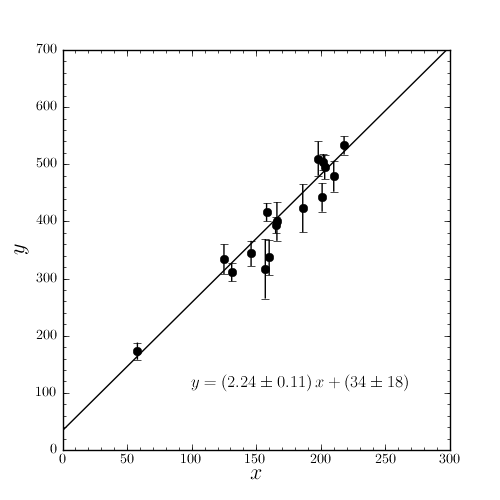
\includegraphics[]{ex1.png}
\caption{Solution to \problemname~\ref{prob:easy}.}\label{fig:easy}
\end{figure}

\clearpage
\begin{figure}[H]
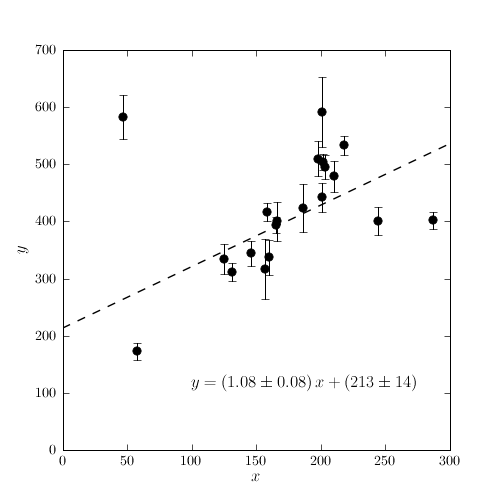
\includegraphics[]{ex2.png}
\caption{Solution to \problemname~\ref{prob:standard}.}\label{fig:standard}
\end{figure}

\clearpage
\begin{figure}[H]
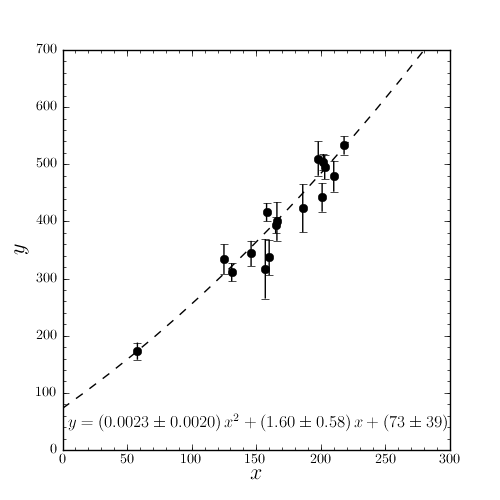
\includegraphics[]{ex3.png}
\caption{Solution to \problemname~\ref{prob:quadratic}.}\label{fig:quadratic}
\end{figure}

\clearpage
\begin{figure}[H]
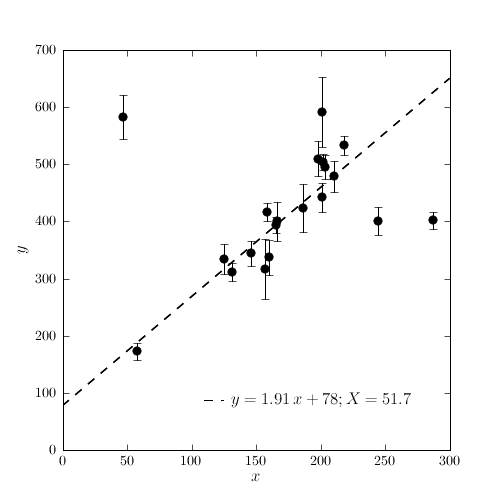
\includegraphics[]{ex6a.png}
\caption{Solution to \problemname~\ref{prob:biexp} using a simple optimizer.}\label{fig:biexpa}
\end{figure}
\clearpage
\begin{figure}[H]
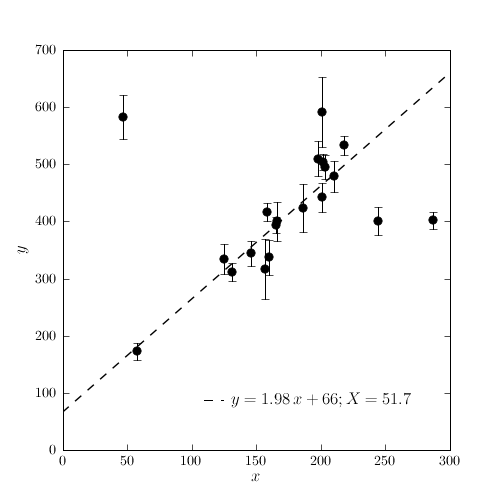
\includegraphics[]{ex6b.png}
\caption{Solution to \problemname~\ref{prob:biexp} using simulated annealing to try to find the global minimum.}\label{fig:biexpb}
\end{figure}
\clearpage
\begin{figure}[H]
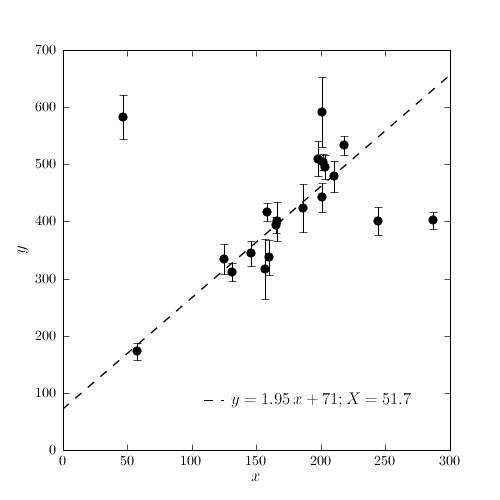
\includegraphics[]{ex6c.png}
\caption{Solution to \problemname~\ref{prob:biexp} using a simple Metropolis sampling scheme.}\label{fig:biexpc}
\end{figure}


\clearpage
\begin{figure}[H]
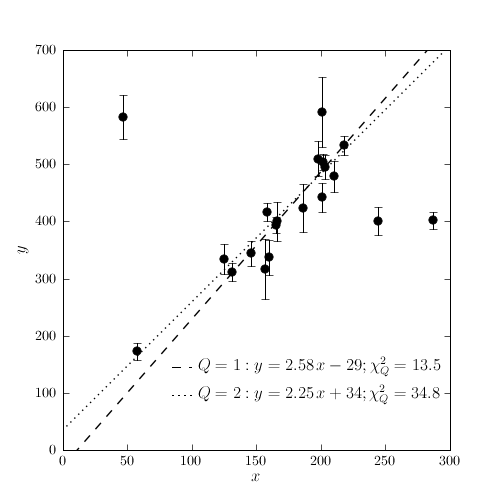
\includegraphics[]{ex7a.png}
\caption{Solution to \problemname~\ref{prob:softchisq} using a simple optimizer.}\label{fig:softchisqa}
\end{figure}
\clearpage
\begin{figure}[H]
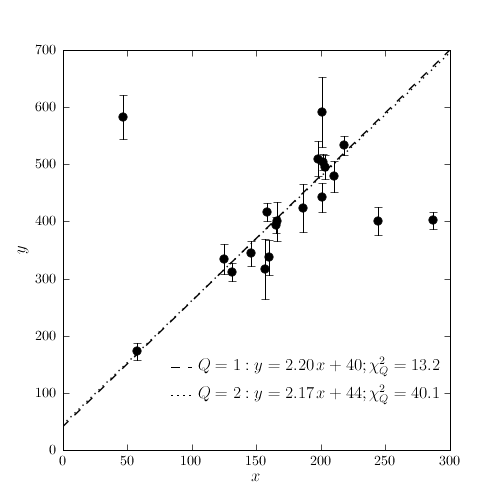
\includegraphics[]{ex7b.png}
\caption{Solution to \problemname~\ref{prob:softchisq} iteratively updating the weights in a regular chi-squared optimization.}\label{fig:softchisqb}
\end{figure}
\clearpage
\begin{figure}[H]
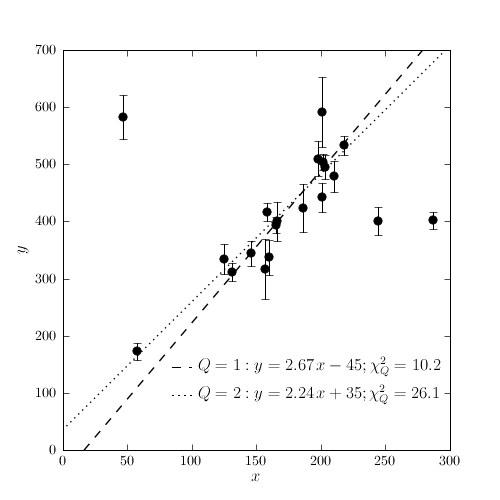
\includegraphics[]{ex7c.png}
\caption{Solution to \problemname~\ref{prob:softchisq} using simulated annealing to try to find the global minimum.}\label{fig:softchisqc}
\end{figure}
\clearpage
\begin{figure}[H]
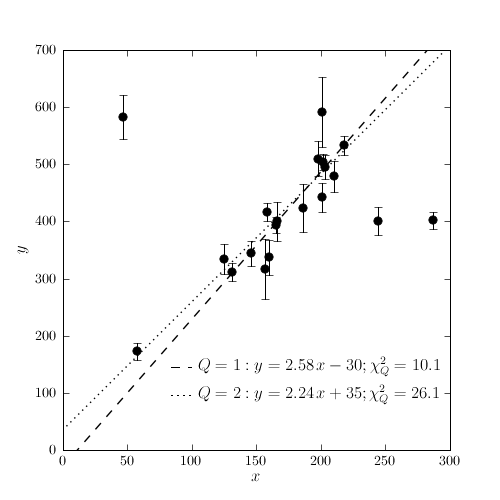
\includegraphics[]{ex7d.png}
\caption{Solution to \problemname~\ref{prob:softchisq} using a simple Metropolis sampling scheme.}\label{fig:softchisqd}
\end{figure}


\clearpage
%Any changes to this table should be made IN THE CODE
\begin{deluxetable}{rrrrrr@{.}l}
\tablecolumns{7}
\tablehead{ID &$x$ & $y$ & $\sigma_y$ & $\sigma_x$ &  \multicolumn{2}{c}{$\rho_{xy}$}}
\tablewidth{0pt}
\startdata
1 & 201 & 592 & 61 & 9 & -0 & 84\\
2 & 244 & 401 & 25 & 4 & 0 & 31\\
3 & 47 & 583 & 38 & 11 & 0 & 64\\
4 & 287 & 402 & 15 & 7 & -0 & 27\\
5 & 203 & 495 & 21 & 5 & -0 & 33\\
6 & 58 & 173 & 15 & 9 & 0 & 67\\
7 & 210 & 479 & 27 & 4 & -0 & 02\\
8 & 202 & 504 & 14 & 4 & -0 & 05\\
9 & 198 & 510 & 30 & 11 & -0 & 84\\
10 & 158 & 416 & 16 & 7 & -0 & 69\\
11 & 165 & 393 & 14 & 5 & 0 & 30\\
12 & 201 & 442 & 25 & 5 & -0 & 46\\
13 & 157 & 317 & 52 & 5 & -0 & 03\\
14 & 131 & 311 & 16 & 6 & 0 & 50\\
15 & 166 & 400 & 34 & 6 & 0 & 73\\
16 & 160 & 337 & 31 & 5 & -0 & 52\\
17 & 186 & 423 & 42 & 9 & 0 & 90\\
18 & 125 & 334 & 26 & 8 & 0 & 40\\
19 & 218 & 533 & 16 & 6 & -0 & 78\\
20 & 146 & 344 & 22 & 5 & -0 & 56\\
\tablecomments{The full uncertainty covariance matrix for each data point is given by\\ $\left[\begin{array}{cc} \sigma_x^2 & \rho_{xy}\sigma_x\sigma_y\\\rho_{xy}\sigma_x\sigma_y & \sigma_y^2\end{array}\right]$.}
\label{table:data_allerr}
\enddata
\end{deluxetable}

\end{document}
